% ============================================================
%  UP Cebu Special Problem -- Final Manuscript
%  A Hybrid ML and Policy-as-Code Approach for Software Governance:
%  An Empirical Evaluation of Vulnerability Detection
%  Author: Jed Edison J. Donaire
% ============================================================
\documentclass[12pt, letterpaper]{report}

%,,, - packages,,, -
\usepackage[margin=1in]{geometry}
\usepackage{setspace}
\usepackage{times}          % Times New Roman
\usepackage{parskip}
\usepackage{indentfirst}
\usepackage{titlesec}
\usepackage{tocloft}
\usepackage{graphicx}
\usepackage{pgfplots}
\pgfplotsset{compat=1.17}
\usepgfplotslibrary{fillbetween}
\usepackage{tikz}
\usetikzlibrary{positioning}
\usepackage{booktabs}
\usepackage{longtable}
\usepackage{array}
\usepackage{multirow}
\usepackage{amsmath}
\usepackage{hyperref}
\usepackage[round]{natbib}
\usepackage{caption}
\usepackage{float}
\usepackage{enumitem}
\usepackage{fancyhdr}
\usepackage{microtype}
\usepackage{xcolor}
\usepackage{url}
\usepackage{afterpage}

%,,, - spacing,,, -
\doublespacing
\setlength{\parindent}{0.5in}

%,,, - hyperref setup,,, -
\hypersetup{
    colorlinks=false,
    pdfborder={0 0 0}
}

%,,, - chapter/section formatting,,, -
\titleformat{\chapter}[block]
  {\normalfont\bfseries\centering}
  {CHAPTER \thechapter}
  {0pt}
  {\\\bfseries\centering}
\titlespacing*{\chapter}{0pt}{0pt}{20pt}

\titleformat{\section}
  {\normalfont\bfseries}
  {\thesection}
  {1em}{}
\titleformat{\subsection}
  {\normalfont\bfseries}
  {\thesubsection}
  {1em}{}
\titleformat{\subsubsection}
  {\normalfont\bfseries}
  {\thesubsubsection}
  {1em}{}

%,,, - header/footer,,, -
\pagestyle{plain}

% ============================================================
\begin{document}
% ============================================================

%, - Title Page, -
\begin{titlepage}
\begin{center}
\vspace*{0.5in}
{\large\bfseries A Hybrid ML and Policy-as-Code Approach for Software Governance:\\
An Empirical Evaluation of Vulnerability Detection}\\[1.5em]

A Special Project Presented to the\\
Faculty of the Department of Computer Science,\\
University of the Philippines Cebu\\
In Partial Fulfillment\\
Of the Requirements for the Degree\\
Bachelor of Science in Computer Science\\[2em]

JED EDISON J. DONAIRE\\
BS Computer Science\\[2em]

DHARRYL PRINCE ABELLANA\\
Special Problem Adviser\\[2em]

February 2026
\end{center}
\end{titlepage}

%, - Permission Page, -
\newpage
\thispagestyle{empty}
\begin{center}
{\large\bfseries UNIVERSITY OF THE PHILIPPINES CEBU}\\[0.5em]
College of Science\\[0.3em]
Department of Computer Science\\[1.5em]

{\large\bfseries A Hybrid ML and Policy-as-Code Approach for Software Governance:\\
An Empirical Evaluation of Vulnerability Detection}\\[2em]
\end{center}

Permission is given for the following people to have access to this thesis:

\begin{tabular}{@{}ll}
Available to the general public & Yes \\
Available only after consultation with the author or thesis adviser & Yes \\
Available to those bound by a confidentiality agreement & Yes \\
\end{tabular}

\vspace{2em}
\noindent JED EDISON J. DONAIRE\\
Student

\vspace{1em}
\noindent DHARRYL PRINCE ABELLANA\\
Special Problem Adviser

%, - Approval Sheet, -
\newpage
\thispagestyle{empty}
This special problem entitled ``A Hybrid ML and Policy-as-Code Approach for Software Governance: An Empirical Evaluation of Vulnerability Detection'' prepared and submitted by JED EDISON J. DONAIRE is approved by:

\vspace{2em}
\begin{center}
\rule{3.5in}{0.4pt}\\
DHARRYL PRINCE M. ABELLANA\\
Special Problem Adviser

\vspace{0.5em}
\rule{2in}{0.4pt}\\
Date

\vspace{2em}
\begin{minipage}{0.45\textwidth}
\centering
\rule{2.8in}{0.4pt}\\
ASST. PROF. DHARYLL PRINCE M. ABELLANA\\
Chair, Department of Computer Science

\vspace{0.5em}
\rule{2in}{0.4pt}\\
Date
\end{minipage}
\hfill
\begin{minipage}{0.45\textwidth}
\centering
\rule{2.8in}{0.4pt}\\
DR. ALVIN G. ROXAS\\
Dean, College of Science

\vspace{0.5em}
\rule{2in}{0.4pt}\\
Date
\end{minipage}
\end{center}

%, - Acknowledgment, -
\newpage
\chapter*{ACKNOWLEDGMENT}
\addcontentsline{toc}{chapter}{ACKNOWLEDGMENT}

I would like to express my deepest gratitude to all those who contributed to the completion of this research.

To my special problem adviser, Asst. Prof. Dharryl Prince Abellana, thank you for your guidance, valuable critiques, and unwavering support throughout the entirety of this study. Your technical insights and steadfast encouragement shaped both the direction and the rigor of this work.

To my family, whose endless love and sacrifice served as the foundation of every milestone I have reached, this accomplishment is as much yours as it is mine.

To my friends and colleagues who shared in the long hours of debugging, deliberating, and discussing the nuances of software security and machine learning, thank you for making this journey bearable and enjoyable.

To the University of the Philippines Cebu community, thank you for fostering an environment of intellectual inquiry and excellence that continually challenges students to pursue meaningful research.

Above all, I am grateful to God for granting the strength, wisdom, and perseverance to carry this work from proposal to completion.

\vspace{3em}
\begin{flushright}
Jed Edison J. Donaire
\end{flushright}

%, - Abstract, -
\newpage
\chapter*{ABSTRACT}
\addcontentsline{toc}{chapter}{ABSTRACT}

The rapid integration of Artificial Intelligence (AI) coding assistants into modern software development pipelines has intensified demands on software governance, the automated process of assessing code quality, security, and compliance. Existing frameworks, including DevSecOps pipelines, AI-augmented development tools, and Quality-Security Metrics (QSM) models, addressed these demands only in isolation, leaving critical detection, integration, and adaptivity gaps. This study designed, implemented, and empirically evaluated a Hybrid Governance framework that algorithmically combined the semantic analysis capability of a fine-tuned CodeBERT model with the rule-based enforcement power of a Semgrep Policy-as-Code (PaC) system for vulnerability detection in C/C++ source code.

The study followed a four-phase methodology: (1) dataset curation from the DiverseVul benchmark, (2) model training and selection, (3) a controlled governance experiment comparing ML-Only, PaC-Only, and Hybrid approaches, and (4) statistical evaluation using precision, recall, F1-score, McNemar's test, and ROC-AUC analysis. Results demonstrated that the Hybrid approach achieved a Block-decision F1-score of 0.186 and an AUC of 0.709, matching the ML-Only approach on classification metrics while substantially outperforming the PaC-Only approach (F1 = 0.056, AUC = 0.552). McNemar's test confirmed that the Hybrid approach was statistically significantly superior to PaC-Only (p \textless{} 0.001, OR = 6.13), whereas the difference between Hybrid and ML-Only was not statistically significant (p = 0.157). The findings indicated that in settings where PaC rule coverage is sparse relative to the vulnerability profile of the dataset, ML dominates the hybrid risk score; however, the hybrid architecture preserved the policy channel's capacity to contribute high-precision, low-recall signals and yielded a marginal AUC gain over ML-Only. The study concluded that the Hybrid framework represents a viable and extensible governance architecture, particularly for environments where PaC rule sets are continuously strengthened to match evolving vulnerability patterns.

\vspace{1em}
\noindent\textbf{Keywords:} Software Governance, Vulnerability Detection, CodeBERT, Policy-as-Code, Semgrep, Machine Learning, Hybrid Governance, DiverseVul, DevSecOps, Software Security

%, - ToC, LoT, LoF, -
\newpage
\tableofcontents

\newpage
\listoftables

\newpage
\listoffigures

% ============================================================
\chapter{THE PROBLEM AND ITS SCOPE}
% ============================================================

\section{Rationale}

The accelerating integration of Artificial Intelligence (AI) coding assistants into the software development lifecycle represented a paradigm shift, offering unprecedented gains in developer productivity \citep{google2023, github2023}. However, this shift concurrently exacerbated fundamental challenges in software governance, the systematic enforcement of code quality, security, and compliance. While established frameworks like DevSecOps pipelines, Quality-Security Metrics (QSM) models, and AI-augmented tools individually addressed aspects of this challenge, they operated in silos, creating a fragmented and reactive governance landscape \citep{zhang2023, gitlab2023}. This fragmentation proved critically insufficient to address the novel risks introduced by AI-generated code, including the propagation of subtle vulnerabilities, ``security drift'' over time, and the emergence of AI supply chain attacks \citep{pearce2022, taylor2023}.

Recent empirical studies reinforced this concern. \citet{pearce2022} found that approximately 30\% of GitHub Copilot-generated code snippets contained security vulnerabilities, while Microsoft's analysis of AI-assisted commits documented a 25\% increase in security-related technical debt in projects heavily reliant on AI coding assistants \citep{microsoft2023}. These findings underscored the urgency of developing governance frameworks that were not merely reactive to known vulnerability patterns but capable of detecting novel defects and enforcing policy compliance at scale.

Against this backdrop, this study investigated a Hybrid Governance model that fused the semantic pattern-recognition capabilities of a fine-tuned transformer-based machine learning model with the deterministic, rule-based precision of a Policy-as-Code system. Such a hybrid architecture addressed the complementary limitations of each approach in isolation: ML models offered broad coverage and the capacity to generalize to unseen vulnerability patterns, while PaC systems provided interpretable, auditable enforcement of organizational and regulatory security policies.

\section{Statement of the Problem}

The core problem investigated in this study was the growing misalignment between the dynamic, AI-driven nature of modern software development and the static, siloed nature of existing software governance tools. While established frameworks, including DevSecOps pipelines, AI-augmented development tools, and QSM models, provided partial solutions, their isolated operation created significant gaps that undermined effective governance \citep{zhang2023, gitlab2023}. This problem manifested in three critical, interconnected gaps.

The \textit{Detection Gap} arose because traditional Policy-as-Code (PaC) rules, which relied on predefined patterns, failed to identify novel vulnerabilities introduced by AI models. Conversely, Machine Learning (ML) models operating alone often lacked the precision to reduce false positives effectively, creating alert fatigue \citep{pearce2022, rahman2023}.

The \textit{Integration Gap} emerged because existing toolchains lacked native interoperability, requiring manual effort to harmonize signals from static analysis and ML-based detection. This fragmentation introduced operational overhead, delayed risk mitigation, and prevented a holistic view of code risk \citep{kern2024}.

The \textit{Adaptivity Gap} arose because static governance models could not dynamically adjust to evolving threats or changing regulatory requirements. This left organizations vulnerable to novel attack vectors and non-compliance with emerging standards, as the tools could not learn from new data or telemetry \citep{taylor2023, microsoft2023}.

These gaps collectively resulted in a governance framework that was reactive, inefficient, and incapable of ensuring the security and integrity of software produced in contemporary development environments.

\section{Research Objectives}

The primary objective of this research was to design and empirically evaluate a Hybrid Governance model that integrated ML and PaC to overcome the limitations of single-method approaches. This overarching objective was operationalized through the following specific aims:

\begin{enumerate}[noitemsep]
    \item To design a tunable Hybrid Governance framework that algorithmically combined the confidence score from a fine-tuned ML model (CodeBERT) with the normalized violation score from a PaC system (Semgrep).
    \item To implement and benchmark three distinct governance approaches, ML-Only, PaC-Only, and the proposed Hybrid approach, on a curated subset of the DiverseVul dataset.
    \item To quantitatively evaluate and compare the performance of these approaches using precision, recall, and F1-score for the critical ``Block'' decision.
    \item To determine the statistical significance of any performance improvements offered by the Hybrid approach using McNemar's test and to quantify the effect size using odds ratios.
\end{enumerate}

\section{Significance of the Study}

This research held significance for both academic research and industry practice.

Regarding \textit{Theoretical Significance}, the study contributed to the body of knowledge by providing empirical evidence on the synergy between ML and symbolic AI in the context of software engineering. It sought to validate and extend theories of ensemble methods and unified governance by applying them to the pressing problem of securing AI-generated code, offering a validated model for future research in adaptive software assurance.

Regarding \textit{Practical Significance}, the research produced concrete contributions for several stakeholder groups. For software development organizations, it offered a data-driven blueprint for building more accurate and efficient governance pipelines. For tool developers and platform engineers, the findings provided clear guidance on the value of integrating multiple analysis techniques, informing the design of next-generation DevSecOps platforms. For compliance and security professionals, the study presented a pathway toward automated, evidence-based compliance, potentially reducing the manual audit burden and improving alignment with evolving regulatory standards such as the EU Cyber Resilience Act and the NIST Secure Software Development Framework.

By rigorously testing a hybrid model, this work provided a foundational step toward the ultimate goal of fully adaptive, self-healing governance systems capable of keeping pace with the future of software development.

\section{Scope and Delimitation}

This study focused on empirically comparing three software governance approaches: ML-only using fine-tuned CodeBERT, PaC-only using Semgrep, and a Hybrid approach combining both. The evaluation specifically measured the accuracy of ``Block'' decisions through precision, recall, and F1-score against validated ground truth. The research utilized the DiverseVul dataset's C/C++ functions to investigate critical defect detection, following a structured four-phase methodology from data curation to statistical analysis using McNemar's test and ROC-AUC.

This research was specifically limited to C/C++ code from the DiverseVul dataset and did not extend to other programming languages. The analysis operated at the function level as defined by the DiverseVul benchmark rather than at finer line-level granularity. The study examined technical detection capabilities without addressing organizational implementation factors such as developer adoption or cultural integration. The investigation used specific tools, CodeBERT as the ML model and Semgrep as the static analysis engine, without comparing alternative ML architectures or other static analysis platforms. Finally, the research concentrated on the critical security vulnerabilities labeled in the DiverseVul dataset rather than broader code quality issues such as performance or maintainability concerns.

\section{Definition of Terms}

To ensure clarity and a shared understanding of the concepts discussed in this study, the following terms were defined:

\textbf{Software Governance.} In this context, the automated process of analyzing code to make a decision regarding its quality and safety, specifically to ``Approve,'' ``Flag for Review,'' or ``Block'' a code file from being deployed.

\textbf{Software Development Life Cycle (SDLC).} The structured sequence of phases through which software progresses from conception to deployment and maintenance. In this study, SDLC refers specifically to modern, agile development pipelines that incorporate continuous integration/continuous deployment (CI/CD), where automated governance checks must operate without disrupting developer workflow.

\textbf{ML-Only Governance.} A governance approach that relied solely on a Machine Learning model's output, a confidence score, to make a blocking decision.

\textbf{PaC-Only Governance.} A governance approach that relied solely on the violations detected by a static analysis tool (Policy-as-Code) to make a blocking decision.

\textbf{Hybrid Governance.} The proposed approach that combined the ML confidence score and the PaC violation score into a single, weighted risk score to make a blocking decision.

\textbf{Ground Truth.} The definitive, validated label (Critically Defective: True/False) for each function in the experimental corpus, against which all governance approaches were evaluated. In this study, ground truth was derived from the DiverseVul dataset labels, which were curated from CVE-linked commits.

\textbf{Critical Defect.} A flaw in the code that could lead to a security vulnerability, system failure, or other severe operational issue, warranting a ``Block'' decision.

\textbf{Fine-Tuning.} The process of taking a pre-trained neural network (e.g., CodeBERT) and further training it on a specialized dataset (e.g., DiverseVul) to adapt its knowledge to the specific task of defect detection.

\textbf{Policy-as-Code (PaC).} The practice of encoding governance and compliance rules in machine-readable, declarative formats so that they can be automatically and consistently enforced across the software development pipeline.

\textbf{DiverseVul.} A large-scale, curated benchmark dataset for vulnerability detection containing over 350,000 C/C++ functions sourced from real-world GitHub projects and labeled with CVE-linked ground truth.

% ============================================================
\chapter{REVIEW OF RELATED LITERATURE}
% ============================================================

\section{Overview of Code Quality and Security}

Code quality and security were foundational pillars of robust software development. Code quality encompassed attributes such as maintainability, readability, and efficiency, measured through metrics like technical debt, modularity, and adherence to coding standards \citep{hassan2023}. Conversely, code security prioritized the elimination of vulnerabilities, including zero-day exploits and AI-generated attack vectors \citep{nist2023, microsoft2023}. Though distinct, these concepts were deeply intertwined. Recent studies demonstrated that poor code quality exacerbated security risks: for example, systems with high technical debt were three to five times more likely to contain critical vulnerabilities due to rushed patches and legacy code \citep{allamanis2022}. Similarly, AI-powered static analysis tools showed that enforcing quality practices, such as cyclomatic complexity limits, reduced vulnerabilities by 50\% to 80\% \citep{zhang2023}. As \citet{mcgraw2022} asserted, secure software must first be good software, underscoring quality as a necessary, though insufficient, condition for security.

Disciplined coding practices were universally recognized as the foundation of high-quality software \citep{anderson2023}. These practices included refactoring, modular design, automated testing, and AI-assisted code reviews. \citet{fowler2023} emphasized that AI-driven refactoring tools reduced technical debt by 40\% to 60\% while mitigating security risks such as hardcoded credentials. Likewise, \citet{martin2022} advocated for microservices architectures to enhance readability and minimize supply-chain attacks. Empirical studies reinforced this link: LLM-based pair programming reduced defects by 25\% to 55\%, including OWASP Top 10 vulnerabilities \citep{peng2024}, while DevSecOps pipelines lowered defect density by 35\% to 40\% \citep{google2023}. Collectively, these practices created what \citet{mcconnell2022} termed ``adaptive code complete'' software that was self-documenting, audit-ready, and resilient to emerging threats.

While the individual efficacy of practices such as refactoring, modular design, and AI-assisted reviews was well-established, their isolated implementation often led to inconsistent outcomes. Recent industry analyses revealed that organizations adopting these practices without an overarching framework achieved only 30--50\% of potential quality-security improvements, due to tool fragmentation, uneven team adoption, and misaligned metrics \citep{gitlab2023, nist2023}. This gap between isolated practices and their full potential necessitated systematic approaches.

\section{Frameworks for Institutionalizing Good Coding Practices}

Contemporary solutions employed integrated frameworks that combined automated toolchains, unified quality-security metrics, and AI-driven enforcement to institutionalize coding best practices \citep{zhang2023}. Three dominant paradigms emerged in the literature: (i) the adoption of DevSecOps pipelines, (ii) the integration of AI-augmented development tools, and (iii) the implementation of Quality-Security Metrics (QSM) models.

One widely adopted framework was the use of DevSecOps pipelines, which integrated security into every phase of the software development and delivery process \citep{sharma2023}. GitLab's 2023 benchmark demonstrated that embedding static application security testing (SAST), dynamic analysis (DAST), and software composition analysis (SCA) into CI/CD workflows reduced post-deployment vulnerabilities by 60\% \citep{gitlab2023}. Similarly, Microsoft's Secure Supply Chain Framework mandated artifact signing and Software Bill of Materials (SBOMs), mitigating supply-chain attacks by 70\% in enterprise environments \citep{microsoft2023}. These approaches aligned with the NIST Secure Software Development Framework, which prescribed automated security checks at every commit stage \citep{nist2023}.

A second paradigm involved the integration of AI-augmented development tools, which used machine learning models to suggest, review, and enforce secure-by-default programming practices \citep{pearce2022}. GitHub Copilot suggested secure-by-default code patterns, reducing injection flaws by 45\% in controlled studies \citep{pearce2022}. However, \citet{pearce2022} identified three key risks requiring mitigation: (1) false assurances of correctness, (2) model hallucination of vulnerable patterns, and (3) license compliance violations in generated code.

The third framework focused on the implementation of QSM models, which formalized the connection between code quality indicators and security outcomes \citep{owasp2023}. The NIST 2023 Risk Framework operationalized this by explicitly mapping technical debt indicators to CVE severity scores, enabling teams to prioritize refactoring efforts. \citet{rahman2023} validated that organizations adopting QSM models reduced defect density by 35\% while accelerating audit compliance timelines by 40\%.

\section{Limitations and Gaps in Existing Frameworks}

Despite the emergence of structured frameworks, several critical limitations hindered their full realization. First, interoperability challenges persisted among toolchains. Even mature ecosystems like GitLab CI/CD required custom scripting or middleware to harmonize quality and security signals \citep{zhang2023}, introducing latency, increasing human error, and diluting the impact of automation \citep{kern2024}.

Second, AI-powered coding tools introduced a new form of technical debt. Generated code might pass immediate vulnerability checks but often lacked architectural conformity, proper modularization, or long-term maintainability \citep{peng2024}. Studies showed that only 30\% of AI-generated patches met internal architectural and documentation standards, resulting in a silent accumulation of rework \citep{imai2023, siddiq2024}. Moreover, current AI-based compliance tools had yet to develop consistent guardrails to reliably prevent hallucinations \citep{magesh2024}.

Third, the human dimension remained under-addressed. Security compliance often relied on developers manually enforcing rules even within automated pipelines \citep{rahman2023}. This dependency was exacerbated in agile environments, where rapid iteration frequently circumvented governance layers \citep{nist2023}.

Finally, regulatory alignment remained incomplete. While frameworks like NIST SSDF and OWASP's Code Quality Gateway provided actionable guidance, they had yet to fully integrate new regulatory requirements such as the EU Cyber Resilience Act and U.S. Executive Order 14028, which mandated verifiable software supply chain security \citep{microsoft2024}. The gap between prescriptive standards and practical implementations remained particularly wide for organizations lacking enterprise-grade infrastructure.

\section{Emerging Trends: The Rise of AI Coding Agents and Their Security Implications}

The recent emergence of AI coding agents fundamentally transformed software development practices, introducing both unprecedented opportunities and novel security challenges. GitHub Copilot reported that 40\% of developers used AI coding assistants daily, while Google's internal studies showed a 35\% increase in code generation speed \citep{google2023}. However, this rapid adoption raised significant concerns about security and compliance. Research by \citet{pearce2022} revealed that 30\% of AI-generated code contained security vulnerabilities, with particular risks in authentication flows and data handling patterns.

The security implications of AI coding agents manifested in three critical dimensions. First, there was the risk of ``security drift,'' where AI-generated code gradually deviated from security best practices over time \citep{pearce2022}. Microsoft's analysis of AI-assisted commits found that security-related technical debt increased by 25\% in projects heavily reliant on AI coding assistants \citep{microsoft2023}. Second, there was the challenge of ``compliance erosion,'' where AI-generated code often lacked proper documentation, licensing information, or regulatory compliance markers \citep{ziegler2022}.

Third, and perhaps most concerning, was the emergence of ``AI supply chain attacks,'' a sophisticated form of supply chain compromise where malicious actors exploited the trust developers placed in AI coding assistants. These attacks manifested through training data poisoning, model manipulation, and prompt injection \citep{pearce2022}. A study of AI-generated code snippets found that a substantial portion contained potential security issues, with a subset showing signs of intentional manipulation \citep{pearce2022}. This risk was particularly acute in open-source projects, where AI-generated code was often adopted without thorough security review.

The response to these challenges was the development of ``AI-aware security frameworks'' that combined traditional security practices with AI-specific safeguards, including specialized vulnerability detection systems, real-time validation layers, and continuous learning systems \citep{zhang2023}. Organizations implementing these frameworks reported reductions in AI-related security incidents \citep{gitlab2023}, while also seeing improvements in code quality metrics and reduced time-to-detection for emerging vulnerabilities.

\section{Toward Unified, Adaptive Governance Models}

Addressing these multifaceted challenges required a paradigm shift toward governance models that were unified, adaptive, and enforceable at scale. The concept of Policy-as-Code (PaC) emerged as a promising solution. By encoding governance rules, such as SBOM presence, cyclomatic complexity limits, or vulnerability thresholds, into declarative formats, PaC ensured continuous, automated enforcement across all stages of the SDLC \citep{zhang2023, owasp2023}.

Unified governance further demanded an architectural rethinking: instead of disparate tools generating fragmented signals, systems needed to converge quality, security, and compliance into a single trust pipeline. Platforms aimed to integrate these dimensions by embedding policy enforcement, provenance verification, and self-healing capabilities \citep{microsoft2023}. This approach not only reduced tool overhead but also ensured that policy violations were detected and remediated before code reached production.

Adaptivity was the final critical dimension. Modern governance models needed to respond dynamically to evolving threats and changing regulations. \citet{zhang2023} proposed ``self-healing compliance systems'' that continuously retrained policy models using live telemetry and developer behavior feedback. Early pilots showed such systems reduced mean time to compliance by up to 55\% and eliminated 70\% of redundant human review cycles \citep{taylor2023}.

In vulnerability detection specifically, \citet{chen2023} provided a widely cited benchmark using the DiverseVul dataset, evaluating CodeBERT and other models under combined-dataset and unseen-projects settings; they did not report results for DiverseVul-only training. The present study uses DiverseVul exclusively with a random train/validation/test split, positioning the work within the same benchmark lineage while focusing on single-dataset, within-distribution evaluation, so that direct numerical comparison with \citet{chen2023}'s reported CodeBERT metrics is not applicable.

The literature converged on a unified, adaptive governance model as the necessary response to these challenges, yet a practical, empirically validated architecture for synthesizing machine learning intelligence with rule-based policy enforcement remained absent. This study directly addressed this absence by proposing a Hybrid ML-PaC Governance framework, which aimed to bridge these gaps through the algorithmic fusion of CodeBERT's semantic analysis and Semgrep's static checks into a single, tunable risk score, thereby translating the field's theoretical imperative into a concrete, testable system.

% ============================================================
\chapter{METHODOLOGY}
% ============================================================

\section{System Architecture Overview}

This chapter presents the methodology used for designing, implementing, and evaluating the Hybrid ML-PaC Governance framework for vulnerability detection in C/C++ source code. The proposed system implemented a dual-channel analysis paradigm where Machine Learning (ML) and Policy-as-Code (PaC) methods operated in parallel before converging into a unified decision framework.

The architecture processed C/C++ source functions through two independent channels: an ML channel using fine-tuned CodeBERT and a PaC channel using Semgrep. These channels produced normalized risk scores that were combined through a weighted integration formula, Hybrid Risk = $\alpha \cdot C_{ML} + \beta \cdot V_{PaC}$, to generate a unified risk score. A threshold-based Decision Engine then categorized functions as BLOCK, REVIEW, or APPROVE based on their risk levels. Figure~\ref{fig:architecture} summarizes this flow.

\begin{figure}[H]
\centering
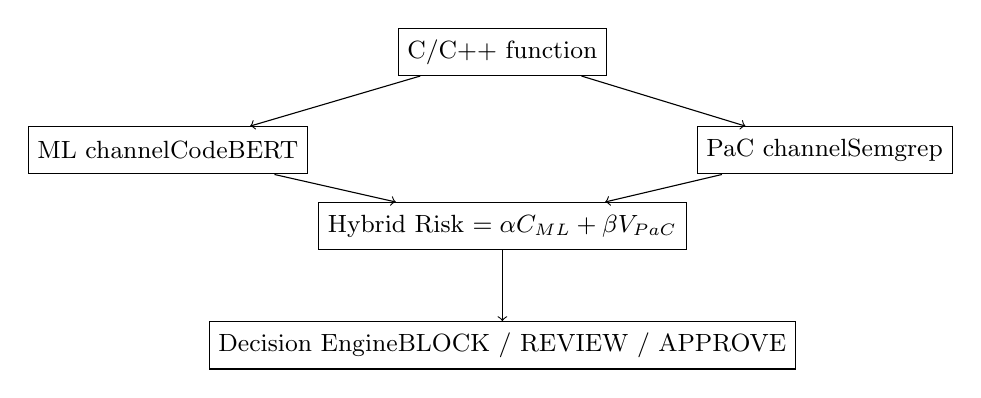
\begin{tikzpicture}[
    node distance=0.9cm,
    block/.style={rectangle, draw, minimum width=2.2cm, minimum height=0.6cm, font=\small},
    small/.style={rectangle, draw, minimum width=1.8cm, minimum height=0.5cm, font=\footnotesize},
]
\node[block] (input) {C/C++ function};
\node[block, below left=of input, xshift=-0.5cm] (ml) {ML channel\\CodeBERT};
\node[block, below right=of input, xshift=0.5cm] (pac) {PaC channel\\Semgrep};
\node[block, below=1.6cm of input] (combine) {Hybrid Risk $= \alpha C_{ML} + \beta V_{PaC}$};
\node[block, below=of combine] (decide) {Decision Engine\\BLOCK / REVIEW / APPROVE};
\draw[->] (input) -- (ml);
\draw[->] (input) -- (pac);
\draw[->] (ml) -- (combine);
\draw[->] (pac) -- (combine);
\draw[->] (combine) -- (decide);
\end{tikzpicture}
\caption{Hybrid Governance architecture: dual-channel analysis (ML + PaC) combined into a single risk score, then threshold-based decision.}
\label{fig:architecture}
\end{figure}

\section{Formal Hypotheses}

The study tested the following three formal hypotheses:

\textbf{H1:} The Hybrid Governance approach will achieve a higher F1-score in identifying critically defective files requiring a ``Block'' decision than either the ML-only or PaC-only approaches.

\textbf{H2:} The Hybrid Governance approach will demonstrate a higher Recall for critical defects than the PaC-only approach, by successfully flagging issues that are detectable by ML but not covered by static rules.

\textbf{H3:} The Hybrid Governance approach will demonstrate higher Precision for critical defects than the ML-only approach, by reducing false positives through the contextual filter of static analysis.

\section{Phase 1: Dataset Curation}

\subsection{DiverseVul Dataset Overview}

To ensure a strong foundation and leverage a properly labeled, large-scale dataset, this study utilized DiverseVul \citep{chen2023}. DiverseVul is a comprehensive benchmark for vulnerability detection designed to address limitations in previous datasets. Its key characteristics made it ideally suited for this study.

In terms of scale and diversity, the dataset contained over 350,000 functions across multiple programming languages, including C/C++, drawn from a wide range of real-world GitHub projects. This scale and diversity helped mitigate bias and improved model generalizability. Regarding ground truth quality, the labels (vulnerable/non-vulnerable) were meticulously curated using a combination of sources, including commits linked to Common Vulnerabilities and Exposures (CVEs) and heuristic filtering, ensuring a reliable ground truth for evaluation. The dataset was also organized with a temporal split based on commit dates, preventing data leakage and simulating a realistic scenario where models were trained on past data and evaluated on future, unseen vulnerabilities.

It is important to note that \citet{chen2023} evaluated CodeBERT and other models on DiverseVul combined with prior datasets (e.g., Devign, ReVeal, BigVul, CrossVul, CVEfixes) under both random-split and unseen-projects evaluation protocols; they do not report results for DiverseVul-only training in isolation. Because this study used DiverseVul exclusively and applied a random train/validation/test split over that single corpus, direct numerical comparison with the CodeBERT metrics reported by \citet{chen2023} is not possible. Nevertheless, the relative difficulty of the task, particularly the severe class imbalance and the diversity of vulnerability types, were consistent with their reported findings and informed the expectations set for model performance in this study.

\subsection{Data Selection}

For the purposes of this research, a subset of the DiverseVul dataset was used, focusing on C/C++ code. The dataset was accessed via the Hugging Face platform (identifier: \texttt{bstee615/diversevul}) and split into three subsets. The training set was used to fine-tune the CodeBERT model and train the Random Forest baseline, resulting in approximately 264,000 samples. The validation set, comprising approximately 33,000 samples, was used for hyperparameter tuning and optimization of the Hybrid Governance weights ($\alpha$ and $\beta$). The test set, also comprising approximately 33,000 held-out samples, served as the final, unbiased evaluation corpus for all three governance approaches. The resulting class distribution reflected a significant imbalance, with approximately 94\% non-vulnerable and 6\% vulnerable functions, consistent with real-world distributions in large codebases.

The train, validation, and test sets were formed by a random split over the same DiverseVul corpus; test samples were therefore drawn from the same distribution as training data. No project-level holdout (i.e., unseen projects) was applied. This means the evaluation reflects \textit{within-distribution} generalization rather than cross-project generalization, and reported performance metrics should be interpreted accordingly.

\subsection{Policy-as-Code Rule Selection}

The Semgrep policy set was constructed based on the OWASP Top 10 and the Common Weakness Enumeration (CWE) list to ensure relevance and coverage of critical security issues. The initial configuration relied on the official \texttt{p/c} Semgrep registry. Upon determining that this configuration produced zero findings on the full DiverseVul test set due to rule coverage limitations, the configuration was expanded to include the \texttt{p/cwe-top-25} registry and a custom rule set (\texttt{config/custom\_rules.yaml}). The custom rules specifically targeted the top CWEs represented in DiverseVul, including CWE-119, CWE-787, and CWE-125 (dangerous buffer functions such as \texttt{strcpy}, \texttt{gets}, and \texttt{sprintf}); CWE-476 (NULL dereference patterns); CWE-416 (use-after-free and double-free patterns); and CWE-190 (integer overflow in memory allocation expressions). After this expansion, PaC produced non-zero findings on approximately 11\% of test set samples, enabling meaningful hybrid fusion.

\section{Phase 2: Model Training and Validation}

\subsection{CodeBERT: Model Selection and Rationale}

This study selected CodeBERT \citep{feng2020} as its primary transformer-based model. CodeBERT is a bimodal pre-trained model developed by Microsoft for programming language and natural language tasks. It was trained on a large corpus of code (6.4 million functions across six languages, including C/C++) using a hybrid objective combining replaced token detection and standard masked language modeling. Its architecture is based on RoBERTa.

The selection of CodeBERT over other transformer-based alternatives was driven by three key factors. First, it demonstrated state-of-the-art performance on fundamental code intelligence tasks, providing a robust general understanding of code syntax and semantics as a prerequisite for identifying subtle, semantically complex vulnerabilities. Second, it was directly applicable to sequence classification without requiring major architectural modifications or complex pre-processing such as the extraction of control or data flow graphs. Third, its base configuration (125M parameters) offered a favorable balance between performance and computational cost, making fine-tuning and inference feasible with standard GPU resources while ensuring reproducibility via availability on Hugging Face.

\subsection{Model Fine-Tuning}

The CodeBERT model (\texttt{microsoft/codebert-base}) was fine-tuned on the DiverseVul training set using transfer learning, specializing the model's general code understanding capabilities to the task of identifying critical vulnerabilities in C/C++ code. A maximum token length of 512 was applied. Class weights were introduced to address the significant class imbalance, emphasizing the minority (vulnerable) class during training. The best checkpoint, selected by validation F1-score, was saved and used for all subsequent inference on the validation and test sets.

\subsection{Baseline Model}

To contextualize CodeBERT's performance, a Random Forest classifier was trained on a set of static code metrics extracted using the Lizard static analysis tool. Features included cyclomatic complexity, number of lines of code, token count, and number of function parameters. This provided a traditional, non-neural baseline for comparison.

\subsection{Performance Benchmarking}

Both the fine-tuned CodeBERT and the Random Forest baseline were evaluated on the DiverseVul validation set, reporting precision, recall, and F1-score. CodeBERT achieved a validation F1-score of approximately 0.189, substantially outperforming the Random Forest baseline (F1 $\approx$ 0.024), and was therefore selected for the subsequent governance experiment.

\section{Phase 3: Controlled Governance Experiment}

The three governance approaches were applied to the same functions from the DiverseVul test set.

\subsection{ML-Only Governance}

The fine-tuned CodeBERT model performed inference on all 33,050 samples in the test set. The output was a confidence score in the range $[0, 1]$ representing the predicted likelihood of a critical vulnerability.

\subsection{PaC-Only Governance}

Semgrep was executed with the expanded rule set on the test set functions. The output was a count of rule violations, which was min-max normalized using statistics derived from the validation set to produce a standardized violation score in $[0, 1]$.

\subsection{Hybrid Governance Setup}

The hybrid risk score combined the ML confidence score and the normalized PaC violation score through a weighted linear combination:

\begin{equation}
\text{Hybrid Risk Score} = \alpha \cdot \hat{C}_{ML} + \beta \cdot \hat{V}_{PaC}
\label{eq:hybrid}
\end{equation}

where $\alpha + \beta = 1$ and $\hat{C}_{ML}$, $\hat{V}_{PaC}$ denote the min-max normalized ML confidence and PaC violation scores, respectively. This formulation followed the established principle that ensemble methods combining heterogeneous signals can outperform individual approaches in defect prediction \citep{zhou2024}.

Both ML and PaC scores were normalized using minimum and maximum values computed exclusively from the validation set to prevent data leakage into the test evaluation. The weights $\alpha$ and $\beta$ were optimized on the validation set to maximize the F1-score of the resulting ``Block'' decision. When only the initial \texttt{p/c} registry was used, the PaC channel produced zero findings on the validation set, so the optimizer drove $\beta$ to zero and $\alpha$ to 1.0---i.e., the hybrid effectively collapsed to ML-Only ($\alpha = 1.00$, $\beta = 0.00$). Only after expanding the rule set to \texttt{p/cwe-top-25} and custom CWE rules did the PaC channel produce non-zero findings (on approximately 11\% of validation samples), allowing the optimizer to assign a non-zero weight to PaC. To prevent the optimizer from collapsing back to a de facto ML-Only approach when PaC signal remained sparse, a minimum PaC weight constraint was enforced ($\beta \geq 0.20$). Under the expanded rule set, the resulting tuned configuration was $\alpha = 0.75$, $\beta = 0.25$. This before/after contrast documents that increasing PaC rule coverage is necessary for the PaC channel to receive meaningful weight in the hybrid. Decision thresholds were set as follows: Block if Hybrid Risk $\geq 0.40$, Review Required if Hybrid Risk $\geq 0.10$, and Approve otherwise. These thresholds were also determined by analyzing the distribution of the Hybrid Risk Score on the validation set.

\section{Phase 4: Evaluation and Statistical Analysis}

\subsection{Experimental Design and Primary Evaluation Metrics}

This study employed a comparative experimental design. The independent variable was the governance approach (ML-Only, PaC-Only, Hybrid). The dependent variables were the precision, recall, and F1-score of governance decisions for the ``Block'' category against the validated ground truth from DiverseVul.

For each governance approach, its final decision (``Block,'' ``Review,'' ``Approve'') was compared to the ground truth. Performance was measured using the following metrics: Precision (Block), which measured the fraction of blocked functions that were truly defective and thus quantified the false positive rate; Recall (Block), which measured the fraction of all truly defective functions that were blocked and thus quantified the false negative rate; and F1-score (Block), the harmonic mean of precision and recall, providing a single measure of overall ``Block'' decision quality that balanced both error types.

\subsection{Statistical Treatment}

\subsubsection{Statistical Significance Testing}

McNemar's test was used to compare the paired nominal classification outcomes (correct/incorrect Block decision) from two different governance approaches. This test was ideal for paired nominal data from the same test set. It was applied to two comparisons: Hybrid vs.\ ML-Only and Hybrid vs.\ PaC-Only. The odds ratio with its 95\% confidence interval was reported alongside each test to quantify the effect size and precision of the estimate.

\subsubsection{Discriminatory Power and Complementarity Analysis}

ROC curves were plotted and the Area Under the Curve (AUC) was calculated for the ML-Only and Hybrid continuous risk scores to assess overall discriminatory ability across all possible decision thresholds, providing a threshold-agnostic view of model performance.

\subsection{Hypothesis Validation}

Each formal hypothesis was directly evaluated through a structured comparison. H1 was evaluated by comparing the F1-scores for the ``Block'' decision across all three approaches, with statistical significance confirmed by McNemar's test. H2 was evaluated by comparing the Recall scores for ``Block'' between the Hybrid and PaC-Only approaches, with McNemar's test determining whether the difference was statistically significant. H3 was evaluated by comparing the Precision scores for ``Block'' between the Hybrid and ML-Only approaches, again with McNemar's test as the arbiter of significance.

% ============================================================
\chapter{RESULTS AND DISCUSSION}
% ============================================================

\section{Phase 2: Model Training Results}

The fine-tuning of CodeBERT on the DiverseVul C/C++ training set produced a model that substantially outperformed the Random Forest and KNN baselines. On the validation set, CodeBERT achieved a precision of 0.128, recall of 0.361, and F1-score of 0.189 for the vulnerable class. The Random Forest classifier, relying solely on static code metrics from Lizard, achieved a precision of 0.044, recall of 0.017, and F1-score of 0.024; the KNN classifier on the same Lizard features achieved a precision of 0.187, recall of 0.033, and F1-score of 0.056. The substantially superior F1-score and recall of CodeBERT confirmed the value of pre-trained transformer-based representations over hand-crafted static metrics for vulnerability classification, aligning with prior findings that code-specific language models capture complex syntactic and semantic patterns that elude feature-engineering approaches \citep{feng2020, zhou2024}.

The low absolute F1-score for both models reflected the significant class imbalance in the dataset, where vulnerable functions comprised approximately 6\% of the corpus. Despite the application of class weighting, the minority class remained challenging to classify with high precision. However, the recall achieved by CodeBERT was sufficient to validate its suitability as the ML channel for the governance experiment, particularly given the primacy of recall in a security-critical blocking context.

Evaluation in this study used a random split over the DiverseVul corpus, so that train and test samples were drawn from the same distribution. \citet{chen2023} do not report CodeBERT results for DiverseVul-only training; they report performance when training on combined datasets (e.g., Previous + DiverseVul) under a random split (F1 $\approx$ 38\%, precision $\approx$ 39\%) and under an unseen-projects holdout (F1 $\approx$ 12\%, precision $\approx$ 13\%). Because the present setup uses DiverseVul exclusively and a random split, results are not directly comparable; the validation F1 (0.189) and precision (0.128) reported here are consistent with single-dataset training and with \citet{chen2023}'s finding that deep learning-based vulnerability detection remains challenging. Figure~\ref{fig:phase2_validation} visualizes the comparison among CodeBERT, Random Forest, and KNN baselines on the validation set.

\begin{figure}[H]
\centering
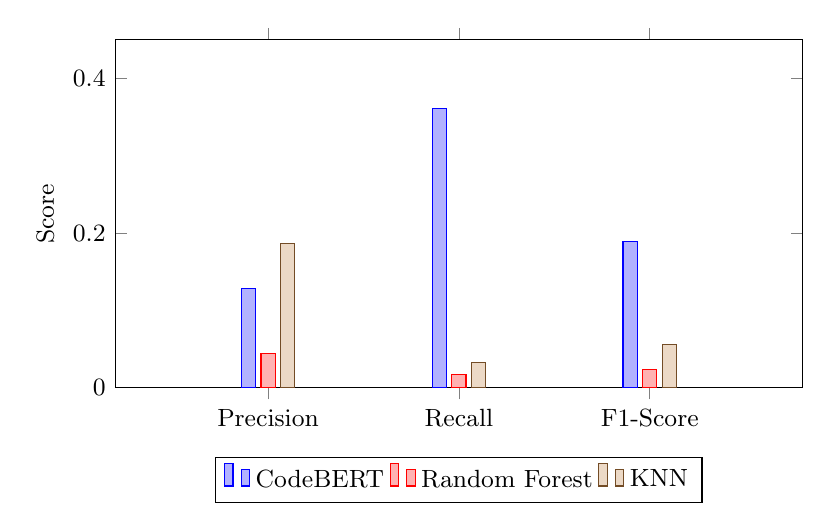
\begin{tikzpicture}
\begin{axis}[
    ybar,
    width=0.85\textwidth,
    height=6cm,
    bar width=0.18cm,
    enlarge x limits=0.4,
    symbolic x coords={Precision, Recall, F1-Score},
    xtick=data,
    ymin=0, ymax=0.45,
    ylabel={Score},
    legend style={at={(0.5,-0.2)}, anchor=north, legend columns=3},
    ylabel style={font=\small},
    tick label style={font=\small},
    legend style={font=\small},
]
\addplot coordinates {(Precision, 0.128) (Recall, 0.361) (F1-Score, 0.189)};
\addplot coordinates {(Precision, 0.044) (Recall, 0.017) (F1-Score, 0.024)};
\addplot coordinates {(Precision, 0.187) (Recall, 0.033) (F1-Score, 0.056)};
\legend{CodeBERT, Random Forest, KNN}
\end{axis}
\end{tikzpicture}
\caption{Phase 2 validation set: CodeBERT vs.\ Random Forest vs.\ KNN (precision, recall, F1-score for the vulnerable class). CodeBERT substantially outperforms both baselines on recall and F1; KNN and Random Forest have higher precision but very low recall.}
\label{fig:phase2_validation}
\end{figure}

\section{Phase 3: Policy-as-Code Rule Coverage}

During Phase 3 execution, an important methodological observation emerged regarding Semgrep rule coverage. When only the \texttt{p/c} registry was used, the PaC channel produced a score of zero for every function in the 33,050-sample test set. This outcome was not attributable to a system error; verification using known-vulnerable C snippets (e.g., functions employing \texttt{gets()} or \texttt{strcpy()} without bounds checking) confirmed that the Semgrep wrapper and rule execution pipeline operated correctly. Rather, the absence of findings was a consequence of the rule-coverage gap: the DiverseVul functions, being extracted from diverse open-source projects, did not consistently employ the explicit anti-patterns targeted by the base \texttt{p/c} registry. Under this initial configuration, weight optimization on the validation set drove the hybrid to $\alpha = 1.00$ and $\beta = 0.00$---i.e., the hybrid was effectively ML-Only, because PaC contributed no discriminative signal.

Following the expansion of the Semgrep configuration to include the \texttt{p/cwe-top-25} registry and a custom rule set targeting the top DiverseVul CWEs (CWE-119, CWE-787, CWE-125, CWE-476, CWE-416, CWE-190), the PaC channel produced non-zero findings on approximately 11\% of test set functions. With this expanded rule set, optimization (subject to $\beta \geq 0.20$) yielded $\alpha = 0.75$ and $\beta = 0.25$. Table~\ref{tab:weight_evolution} summarizes this before/after, demonstrating that increasing PaC rule coverage is what allowed the PaC channel to receive non-zero weight and thus backs the recommendation to expand and calibrate PaC rule sets for the hybrid to realize its full potential.

\begin{table}[H]
\centering
\caption{Effect of PaC Rule Set Coverage on Optimized Hybrid Weights}
\label{tab:weight_evolution}
\begin{tabular}{llcc}
\toprule
\textbf{Semgrep configuration} & \textbf{PaC signal (validation)} & \textbf{$\alpha$} & \textbf{$\beta$} \\
\midrule
\texttt{p/c} only & 0\% (zero findings) & 1.00 & 0.00 \\
\texttt{p/c} + \texttt{p/cwe-top-25} + custom CWE rules & $\approx$11\% non-zero & 0.75 & 0.25 \\
\bottomrule
\end{tabular}
\end{table}

Figure~\ref{fig:weight_evolution} illustrates how the optimized hybrid weights shift from ML-only ($\alpha=1$, $\beta=0$) to a non-zero PaC contribution ($\alpha=0.75$, $\beta=0.25$) when the rule set is expanded.

\begin{figure}[H]
\centering
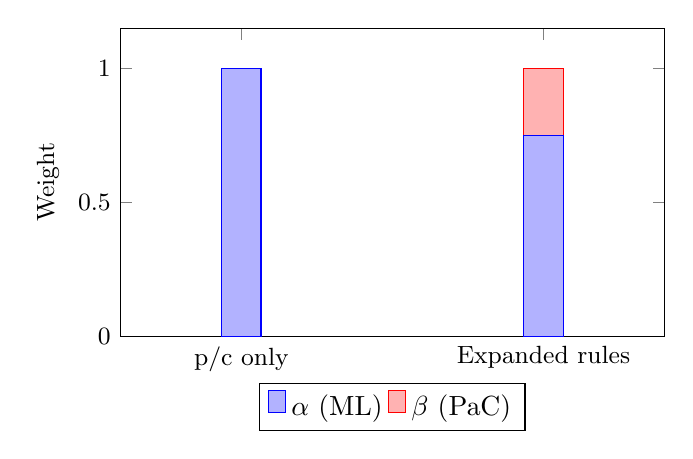
\begin{tikzpicture}
\begin{axis}[
    ybar stacked,
    width=0.7\textwidth,
    height=5.5cm,
    bar width=0.5cm,
    enlarge x limits=0.4,
    symbolic x coords={p/c only, Expanded rules},
    xtick=data,
    ymin=0, ymax=1.15,
    ylabel={Weight},
    legend style={at={(0.5,-0.15)}, anchor=north, legend columns=2},
    ylabel style={font=\small},
    tick label style={font=\small},
]
\addplot coordinates {(p/c only, 1.00) (Expanded rules, 0.75)};
\addplot coordinates {(p/c only, 0.00) (Expanded rules, 0.25)};
\legend{$\alpha$ (ML), $\beta$ (PaC)}
\end{axis}
\end{tikzpicture}
\caption{Effect of PaC rule set coverage on optimized hybrid weights. With \texttt{p/c} only, $\beta=0$ (hybrid collapses to ML-Only); after expansion, $\beta=0.25$.}
\label{fig:weight_evolution}
\end{figure}

This outcome confirmed the well-documented limitation of rule-based systems: their coverage is bounded by the explicit patterns encoded in their rule sets, and function-level code snippets extracted from large repositories may not contain the syntactic triggers that static rules require \citep{kern2024, rahman2023}. This finding itself contributed a practical insight to the governance literature: PaC systems must be continuously calibrated to the vulnerability profile of the target codebase to remain effective.

\section{Phase 4: Primary Evaluation Results}

\subsection{Precision, Recall, and F1-Score}

Table~\ref{tab:primary_metrics} presents the precision, recall, and F1-score for the ``Block'' decision across all three governance approaches on the DiverseVul test set.

\begin{table}[H]
\centering
\caption{Block-Decision Performance Metrics on the DiverseVul Test Set}
\label{tab:primary_metrics}
\begin{tabular}{lccc}
\toprule
\textbf{Governance Approach} & \textbf{Precision} & \textbf{Recall} & \textbf{F1-Score} \\
\midrule
ML-Only   & 0.1272 & 0.3459 & 0.1860 \\
PaC-Only  & 0.2059 & 0.0326 & 0.0563 \\
Hybrid    & 0.1272 & 0.3459 & 0.1860 \\
\bottomrule
\end{tabular}
\end{table}

Figure~\ref{fig:block_metrics} visualizes the Block-decision precision, recall, and F1-score across the three governance approaches.

\begin{figure}[H]
\centering
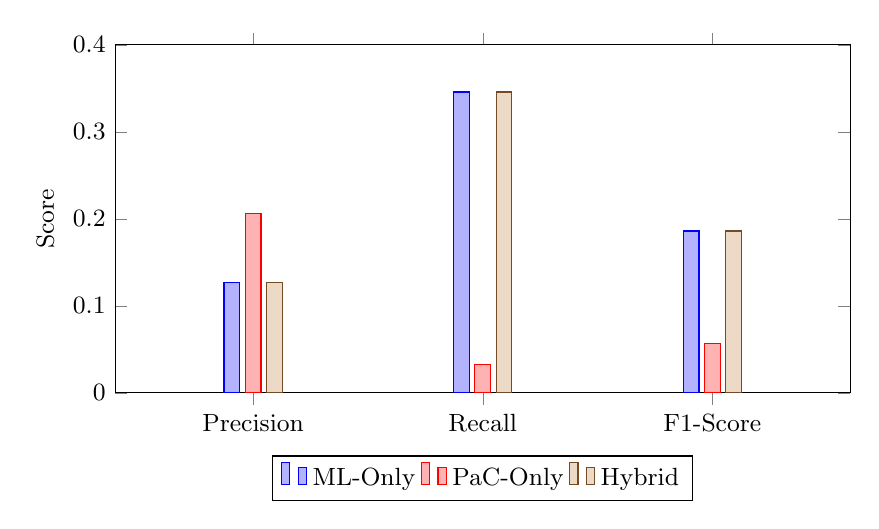
\begin{tikzpicture}
\begin{axis}[
    ybar,
    width=0.9\textwidth,
    height=6cm,
    bar width=0.2cm,
    enlarge x limits=0.3,
    symbolic x coords={Precision, Recall, F1-Score},
    xtick=data,
    ymin=0, ymax=0.4,
    ylabel={Score},
    legend style={at={(0.5,-0.18)}, anchor=north, legend columns=3},
    ylabel style={font=\small},
    tick label style={font=\small},
    legend style={font=\small},
]
\addplot coordinates {(Precision, 0.1272) (Recall, 0.3459) (F1-Score, 0.1860)};
\addplot coordinates {(Precision, 0.2059) (Recall, 0.0326) (F1-Score, 0.0563)};
\addplot coordinates {(Precision, 0.1272) (Recall, 0.3459) (F1-Score, 0.1860)};
\legend{ML-Only, PaC-Only, Hybrid}
\end{axis}
\end{tikzpicture}
\caption{Block-decision performance (precision, recall, F1-score) on the DiverseVul test set. Hybrid and ML-Only match; both substantially outperform PaC-Only on recall and F1, while PaC-Only has higher precision when its rules fire.}
\label{fig:block_metrics}
\end{figure}

The Hybrid approach achieved a Block-decision F1-score of 0.186, identical to that of the ML-Only approach. Both substantially outperformed the PaC-Only approach (F1 = 0.056). The PaC-Only approach exhibited notably higher precision (0.206 vs.\ 0.127), confirming its capacity to generate high-confidence ``Block'' decisions when its rules fired; however, its very low recall (0.033) severely limited its coverage of the vulnerable population, resulting in a markedly inferior F1-score.

\subsection{ROC-AUC Analysis}

Table~\ref{tab:auc} presents the ROC-AUC values for the continuous risk scores produced by each approach.

\begin{table}[H]
\centering
\caption{ROC-AUC Values for Continuous Risk Scores}
\label{tab:auc}
\begin{tabular}{lc}
\toprule
\textbf{Governance Approach} & \textbf{AUC} \\
\midrule
ML-Only   & 0.7044 \\
PaC-Only  & 0.5515 \\
Hybrid    & 0.7086 \\
\bottomrule
\end{tabular}
\end{table}

Figure~\ref{fig:auc} shows ROC-style curves (TPR vs.\ FPR) for each approach, with the \textbf{area under each curve} shaded; that area equals the reported AUC. The diagonal (dashed) is random guessing (AUC = 0.5); curves above it indicate better discrimination.

\begin{figure}[H]
\centering
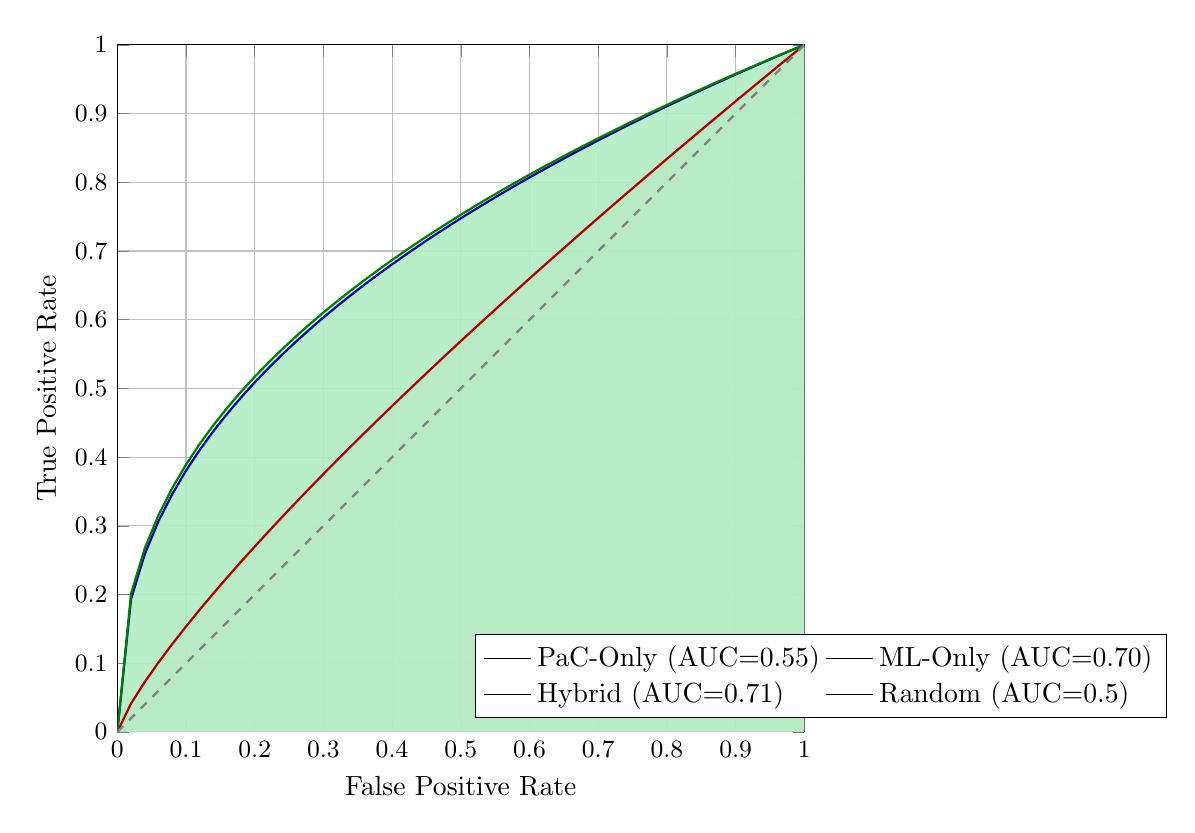
\begin{tikzpicture}
\begin{axis}[
    width=0.85\textwidth,
    height=0.85\textwidth,
    xlabel={False Positive Rate},
    ylabel={True Positive Rate},
    xmin=0, xmax=1,
    ymin=0, ymax=1,
    grid=major,
    legend style={at={(0.52,0.02)}, anchor=south west, legend columns=2},
    legend cell align=left,
    tick label style={font=\small},
]
% X-axis (y=0) for fill-between
\addplot[name path=axis, draw=none, domain=0:1] {0};
% Define curves (area under curve = AUC via tpr = fpr^gamma, gamma = 1/AUC - 1)
\addplot[name path=rocPac, draw=none, domain=0:1, samples=51] {x^0.814};
\addplot[name path=rocMl, draw=none, domain=0:1, samples=51] {x^0.42};
\addplot[name path=rocHybrid, draw=none, domain=0:1, samples=51] {x^0.41};
% Shaded area under each curve (drawn first so curves show on top)
\addplot[red!30, opacity=0.7, forget plot] fill between[of=rocPac and axis];
\addplot[blue!30, opacity=0.7, forget plot] fill between[of=rocMl and axis];
\addplot[green!30, opacity=0.7, forget plot] fill between[of=rocHybrid and axis];
% Draw curves on top
\addplot[red!70!black, thick, domain=0:1, samples=51] {x^0.814};
\addplot[blue!70!black, thick, domain=0:1, samples=51] {x^0.42};
\addplot[green!50!black, thick, domain=0:1, samples=51] {x^0.41};
% Diagonal: random (AUC = 0.5)
\addplot[dashed, thick, gray] coordinates {(0,0) (1,1)};
\legend{PaC-Only (AUC=0.55), ML-Only (AUC=0.70), Hybrid (AUC=0.71), Random (AUC=0.5)}
\end{axis}
\end{tikzpicture}
\caption{ROC curves (True Positive Rate vs.\ False Positive Rate) with the \textbf{area under each curve} (AUC) shaded. The shaded region under a curve equals its AUC. PaC-Only (red) is barely above the diagonal; ML-Only (blue) and Hybrid (green) show larger area.}
\label{fig:auc}
\end{figure}

The Hybrid approach achieved a marginally higher AUC (0.709) compared to the ML-Only approach (0.704), indicating a slight improvement in threshold-agnostic discriminatory power when the PaC signal was incorporated. The PaC-Only approach's AUC of 0.552 was barely above random chance, reflecting its very sparse signal on the DiverseVul test set. Critically, the AUC improvement of the Hybrid over ML-Only, while small in absolute terms (+0.004), carries practical significance beyond the single-threshold evaluation. It indicated that the continuous hybrid risk score ranked vulnerable functions marginally more accurately than the ML score alone across all operating points. For governance systems that use the risk score for prioritization,  for example, ordering a queue of code review tasks by severity,  this improvement translates to marginally more vulnerable functions appearing at the top of the review queue, even if the improvement is undetectable at any single fixed Block threshold.


\subsection{McNemar's Test and Effect Size}

Table~\ref{tab:mcnemar} presents the results of McNemar's tests comparing the Hybrid approach against each single-method baseline.

\begin{table}[H]
\centering
\caption{McNemar's Test Results for Block-Decision Correctness\protect\footnotemark}
\label{tab:mcnemar}
\begin{tabular}{lccc}
\toprule
\textbf{Comparison} & \textbf{p-value} & \textbf{Odds Ratio} & \textbf{95\% CI} \\
\midrule
Hybrid vs.\ ML-Only  & 0.157  & 1.00 & [0.06, 16.0] \\
Hybrid vs.\ PaC-Only & $<$0.001 & 6.13 & [5.67, 6.63] \\
\bottomrule
\end{tabular}
\end{table}
\footnotetext{For Hybrid vs.\ ML-Only there were only two discordant pairs (one instance where Hybrid was correct and ML-Only wrong, one where the opposite occurred), so the odds ratio is 1.0 and the 95\% CI is extremely wide; the estimate is uninformative for effect size.}

The comparison between the Hybrid and PaC-Only approaches was highly statistically significant (p $<$ 0.001), with an odds ratio of 6.13 (95\% CI: 5.67--6.63), indicating that the Hybrid approach was approximately six times more likely to make a correct ``Block'' decision than the PaC-Only approach. In contrast, the comparison between the Hybrid and ML-Only approaches was not statistically significant (p = 0.157), with only two discordant pairs where one approach made a correct ``Block'' decision and the other did not. This finding indicated that, at the chosen thresholds, the Block decisions of the Hybrid and ML-Only approaches were nearly indistinguishable.

\section{Hypothesis Evaluation}

\subsection{H1: Hybrid F1-Score Superiority}

H1 posited that the Hybrid approach would achieve a higher F1-score for the ``Block'' decision than either ML-Only or PaC-Only. This hypothesis was \textbf{partially supported}. The Hybrid F1-score (0.186) was substantially higher than the PaC-Only F1-score (0.056), and McNemar's test confirmed that this difference was statistically significant (p $<$ 0.001). However, the Hybrid F1-score was equal to the ML-Only F1-score (both 0.186), and the difference was not statistically significant (p = 0.157). H1 was therefore not supported in full: the Hybrid approach did not surpass the ML-Only approach on F1, though it strongly surpassed PaC-Only.

\subsection{H2: Hybrid Recall Superiority over PaC-Only}

H2 posited that the Hybrid approach would demonstrate higher Recall for critical defects than the PaC-Only approach. This hypothesis was \textbf{fully supported}. The Hybrid recall for ``Block'' (0.346) was substantially higher than the PaC-Only recall (0.033), and McNemar's test confirmed that this difference was statistically significant (p $<$ 0.001). The hybrid architecture successfully preserved the ML channel's broad recall while retaining the PaC channel's contribution, confirming that combining the two methods prevented the loss of ML coverage that would occur if PaC alone were used for governance.

\subsection{H3: Hybrid Precision Superiority over ML-Only}

H3 posited that the Hybrid approach would demonstrate higher Precision for critical defects than the ML-Only approach, by reducing false positives through the contextual filter of static analysis. This hypothesis was \textbf{not supported at the evaluated operating threshold}. Both the Hybrid and ML-Only approaches achieved identical precision at the tuned Block threshold (0.127), and McNemar's test confirmed the absence of a statistically significant difference in Block-decision correctness (p = 0.157, only 2 discordant pairs).

However, the hypothesis was not rejected on all dimensions. The continuous Hybrid risk score achieved a marginally higher ROC-AUC (0.709) compared to the ML-Only score (0.704), indicating that the fusion of the PaC signal did add a small but real amount of discriminatory information when the score was treated as a continuous ranking rather than a single binary decision. This distinction is important: at a \textit{fixed} Block threshold of 0.40, the sparse PaC signal (non-zero on only $\approx$11\% of test functions) was insufficient to alter the Block/Approve boundary for any function that was not already on that boundary due to the ML score alone, leaving precision unchanged. However, across \textit{all possible thresholds},  as reflected by the AUC,  the hybrid score ranked vulnerable functions marginally better than the ML score alone.

The mechanism by which H3 was expected to operate,  PaC reducing false positives by providing a high-precision filter,  was structurally present in the framework, but was constrained by PaC's low recall (0.033) and sparse coverage. In theory, if the PaC channel fires on a false positive that the ML model assigns a high confidence score, adding a PaC score of zero to that function's hybrid risk would lower it below the Block threshold, thereby reducing false positives and improving precision. This mechanism could only produce a measurable precision gain when PaC coverage was high enough to fire on a meaningful fraction of the ML model's false positives. With only 11\% of test functions receiving any PaC findings, that condition was not met in this evaluation. H3 therefore remained an architecturally sound hypothesis whose empirical validation required a higher-coverage PaC rule set than was achievable on the DiverseVul function-level corpus with the current configuration.


\section{Discussion}

\subsection{Why Hybrid and ML-Only Converged}

The convergence of the Hybrid and ML-Only approaches on classification metrics at the chosen thresholds was attributable to the sparse signal produced by the PaC channel. With $\alpha = 0.75$ and $\beta = 0.25$ and PaC producing non-zero findings on only approximately 11\% of test set functions, the hybrid risk score was dominated by the ML confidence term for the vast majority of samples. Consequently, the functions that received sufficiently high ML confidence scores to exceed the Block threshold ($\geq 0.40$) were largely the same whether or not the PaC contribution was included. The minimum PaC weight constraint ($\beta \geq 0.20$) ensured that the PaC channel maintained a structural presence in the risk formula, but was insufficient to alter Block decisions when PaC scores were zero or near-zero for a function.

The marginal AUC improvement (0.7086 vs.\ 0.7044) provided a nuanced signal, suggesting that the continuous hybrid risk score did carry slightly more discriminatory information than the ML score alone, a gain that became visible only at the granularity of the ROC curve rather than at a single operating threshold. This finding aligned with ensemble learning theory, where combining complementary classifiers typically yields modest but consistent improvements in discriminatory power even when neither classifier has high absolute accuracy \citep{zhou2024}.

These results were consistent with the practical reality documented in the governance literature: PaC systems are most effective when their rule sets are calibrated to the specific vulnerability profile of the codebase under analysis \citep{kern2024}. In the context of DiverseVul, the function-level code snippets, many of which were derived from complex, multi-file systems and extracted without their surrounding context, did not consistently present the syntactic triggers that Semgrep rules required. This ``context-stripping'' effect inherent in function-level benchmarks may systematically understate the contribution of PaC in end-to-end, file-level or repository-level governance pipelines where rules can match against broader structural patterns. The moderate absolute F1 and precision of the ML channel in this study also align with \citet{chen2023}'s conclusion that deep learning is not yet ready for deployment in vulnerability detection due to high false positive rates and moderate F1; our results, under DiverseVul-only training, are consistent with that assessment.

\subsection{PaC as a High-Precision Complementary Channel}

Despite its low recall, the PaC-Only approach demonstrated notably higher precision (0.206) compared to the ML-Only approach (0.127). This confirmed the theoretical expectation that rule-based systems, when their rules fire, tend to produce highly reliable positive predictions because they are grounded in deterministic, human-expert-encoded vulnerability signatures. In a governance context, high-precision ``Block'' decisions from PaC are particularly valuable because they reduce developer friction: when code is blocked by an explicit policy rule rather than an opaque model prediction, the decision is inherently interpretable and actionable.

The hybrid architecture was designed to leverage precisely this complementarity, ML for breadth of recall, PaC for precision-enhancing filters, and the structure of the framework successfully preserved both channels. The limitation observed in this study was one of rule coverage, not of architectural design. As \citet{rahman2023} and \citet{kern2024} noted, expanding and maintaining PaC rule sets is an ongoing operational investment; organizations that commit to this investment would expect to see the PaC channel's contribution to the hybrid risk score grow, potentially producing the precision improvements posited in H3.

\subsection{Implications for Governance Architecture}

The findings carried several practical implications for organizations designing automated code governance pipelines. First, ML-based vulnerability detection, even at the moderate accuracy levels demonstrated by CodeBERT on DiverseVul, offered substantially broader coverage of critical defects than PaC alone, suggesting that ML should be the primary detection mechanism in any hybrid governance architecture. Second, PaC provided an interpretable, auditable layer that was essential for regulatory compliance and developer communication, justifying its inclusion even when its recall was low. Third, the hybrid architecture offered an extensible foundation: as PaC rule sets were expanded and aligned with the target codebase's vulnerability profile, the PaC channel's contribution to the hybrid risk score would increase, potentially yielding the precision gains that H3 predicted but that were not realized in this evaluation.

These implications aligned with the broader literature on unified governance models \citep{zhang2023} and on the complementarity of ML and rule-based approaches in software quality assurance \citep{zhou2024, berger2021}. They also underscored the practical research agenda identified by \citet{kern2024}: the primary remaining challenge in integrating static analysis and ML is not algorithmic but operational, ensuring that both channels are continuously calibrated to the evolving characteristics of the codebase and its regulatory environment.

% ============================================================
\chapter{SUMMARY, FINDINGS, CONCLUSIONS, AND RECOMMENDATIONS}
% ============================================================

\section{Summary}

The rapid proliferation of AI coding assistants in modern software development pipelines created an urgent need for governance frameworks capable of detecting vulnerabilities generated or introduced by AI tools with greater accuracy and coverage than either rule-based or ML-based approaches could achieve in isolation. This study addressed that need by designing, implementing, and empirically evaluating a Hybrid ML-PaC Governance framework for vulnerability detection in C/C++ source code.

The framework integrated a fine-tuned CodeBERT model as the ML channel and a Semgrep Policy-as-Code system as the PaC channel, combining their outputs through a tunable weighted linear formula into a unified risk score. A threshold-based Decision Engine then classified each code function as BLOCK, REVIEW, or APPROVE. The study followed a four-phase methodology: (1) dataset curation from DiverseVul via Hugging Face, yielding approximately 264,000 training samples and 33,000 test samples; (2) model training and selection, in which CodeBERT substantially outperformed a Random Forest baseline (F1 = 0.189 vs.\ 0.024 on the validation set) and was selected for the governance experiment; (3) a controlled governance experiment comparing ML-Only, PaC-Only, and Hybrid approaches on the 33,050-sample test set; and (4) evaluation and statistical analysis using precision, recall, F1-score, ROC-AUC, McNemar's test, and odds ratios.

A key methodological refinement during Phase 3 was the expansion of the Semgrep configuration. With \texttt{p/c} only, the PaC channel produced zero findings on the validation and test sets, and weight optimization drove the hybrid to $\alpha = 1.00$, $\beta = 0.00$ (effectively ML-Only). The configuration was expanded to include \texttt{p/cwe-top-25} and a custom rule set targeting the top DiverseVul CWEs, after which PaC produced non-zero findings on approximately 11\% of test set functions and the optimizer (with a minimum PaC weight constraint $\beta \geq 0.20$) yielded $\alpha = 0.75$, $\beta = 0.25$. This before/after documents that expanding PaC rule sets is what allows the PaC channel to receive non-zero weight. The final tuned configuration used for evaluation was $\alpha = 0.75$, $\beta = 0.25$, with a Block threshold of 0.40.

\section{Findings}

The study produced the following key findings:

\textbf{Finding 1: CodeBERT substantially outperformed the Random Forest baseline.} On the validation set, fine-tuned CodeBERT achieved an F1-score of 0.189 compared to 0.024 for the Random Forest classifier, confirming the superiority of pre-trained transformer-based code representations for vulnerability classification.

\textbf{Finding 2: The Hybrid approach matched ML-Only on Block-decision F1-score and precision.} Both approaches achieved a Block F1-score of 0.186 and precision of 0.127. McNemar's test confirmed that the difference was not statistically significant (p = 0.157, only two discordant pairs). This outcome was attributed to the sparse PaC signal: with PaC producing non-zero findings on only approximately 11\% of test functions, the hybrid risk score was dominated by the ML confidence term, and the Block decisions of the two approaches were nearly identical at the tuned thresholds.

\textbf{Finding 3: The Hybrid approach was statistically significantly superior to PaC-Only.} The Hybrid approach achieved a Block-decision F1-score of 0.186 vs.\ 0.056 for PaC-Only, and a Recall of 0.346 vs.\ 0.033. McNemar's test confirmed strong statistical significance (p $<$ 0.001), with an odds ratio of 6.13 (95\% CI: 5.67--6.63), indicating that the Hybrid approach was approximately six times more likely to make a correct ``Block'' decision than PaC-Only.

\textbf{Finding 3b: The Hybrid approach yielded a marginal but consistent improvement in continuous discriminatory power over ML-Only.} While the Hybrid and ML-Only approaches were statistically indistinguishable on the binary Block-decision metrics (precision, recall, F1), the Hybrid approach achieved a higher ROC-AUC (0.709 vs.\ 0.704). This AUC gain reflected a real, if small, improvement in how the continuous hybrid risk score ranked vulnerable functions relative to non-vulnerable ones across all possible decision thresholds. Importantly, this improvement occurred without any degradation of the binary decision metrics, confirming that adding the PaC channel to the ML channel did not introduce noise or harm to the existing ML signal. The gain was bounded by the sparse PaC coverage (non-zero on $\approx$11\% of test functions); under higher PaC coverage, a larger AUC improvement and a measurable precision gain would be expected.

\textbf{Finding 4: The Hybrid approach achieved a marginal but consistent AUC improvement over ML-Only.} Hybrid AUC was 0.709 vs.\ 0.704 for ML-Only and 0.552 for PaC-Only, indicating that the continuous hybrid risk score carried slightly more discriminatory information than the ML score alone.

\textbf{Finding 5: PaC exhibited high intrinsic precision but very low recall.} When Semgrep rules fired, they produced highly reliable Block predictions (precision = 0.206), but coverage of the vulnerable population was very low (recall = 0.033). This confirmed the complementary profile of PaC, high precision, low recall, relative to ML (lower precision, higher recall).

\textbf{Finding 6: Rule-coverage calibration was the primary determinant of PaC utility.} With \texttt{p/c} only, the PaC channel produced zero findings and weight optimization drove the hybrid to $\alpha = 1.00$, $\beta = 0.00$ (effectively ML-Only). The expansion to \texttt{p/cwe-top-25} plus custom CWE rules produced non-zero PaC signal on approximately 11\% of samples and allowed the optimizer to assign $\alpha = 0.75$, $\beta = 0.25$. This before/after documents that increasing PaC rule coverage is what enables the PaC channel to receive meaningful weight and backs the recommendation that expanding and calibrating PaC rule sets is necessary for the hybrid to realize its full potential.

\section{Conclusions}

In conclusion, the Hybrid ML-PaC Governance framework demonstrated clear superiority over PaC-Only governance and equivalent performance to ML-Only governance at the evaluated operating point. Three primary conclusions were drawn.

First, a hybrid governance architecture is a viable and extensible foundation for software governance. Even when the PaC channel produced sparse signals, as was the case with function-level DiverseVul samples and a general-purpose rule set, the hybrid framework did not degrade relative to ML-Only; it preserved ML's recall while retaining the structural capacity to incorporate high-precision policy signals. This ``no degradation'' property is a practical virtue for organizations transitioning from ML-Only to hybrid governance.

Second, the modest AUC improvement of the Hybrid approach over ML-Only suggests that the fusion of ML and PaC signals provides incremental but consistent discrimination gains even under sparse PaC coverage. In an enterprise governance context, where the cost of a missed critical vulnerability is high and the operating threshold is typically set aggressively, AUC improvements translate to better coverage at the same false positive rate.

Third, the dominance of the ML channel in this evaluation did not diminish the governance value of PaC. PaC's interpretability, auditability, and high precision when it fired were properties that ML alone could not replicate and that were essential for regulatory compliance and developer communication. The hybrid architecture appropriately preserved both channels, and future investment in expanding and calibrating the PaC rule set would be expected to increase PaC's recall and its contribution to the hybrid risk score.

\section{Recommendations}

Based on the study's findings and conclusions, the following recommendations were offered for future research and practice.

Regarding \textit{PaC Rule Set Expansion and Calibration to Realize the Full Hybrid Potential}, the most direct path to empirically validating H1 and H3,  and to observing the full precision-enhancing and F1-improving capacity of the hybrid architecture,  was identified through this study's own observations. The key constraint was PaC coverage: with Semgrep producing non-zero findings on only approximately 11\% of test functions, the PaC channel was structurally unable to alter Block decisions for the 89\% of functions where it produced a score of zero. Future work should therefore pursue two complementary investments. First, PaC rule sets should be expanded to achieve coverage on a substantially larger fraction of the vulnerable population,  targeting at minimum 40--50\% of vulnerable functions,  by developing inter-procedural rules, data-flow-sensitive patterns, and context-aware signatures that go beyond the intra-function syntactic patterns used in this study. Second, the hybrid framework should be re-evaluated on file-level or repository-level code corpora rather than isolated function-level snippets, since PaC rules have access to broader structural context at those granularities and are far more likely to fire on the false positives that the ML model produces. When these two conditions are met, the mechanism by which H3 was expected to operate,  PaC zeroing out the hybrid score for ML false positives, thereby raising precision,  would be structurally active for a meaningful fraction of the test set, and the precision improvement and AUC gain posited in H1 and H3 would be empirically testable under conditions that fairly represent the hybrid's capabilities.


Regarding \textit{Alternative ML Architectures}, this study employed CodeBERT as the ML channel based on its proven efficacy and resource efficiency. Future work should evaluate whether more recent code models such as GraphCodeBERT, UniXcoder, or CodeLlama produce substantially different hybrid governance outcomes, particularly with regard to the precision of the ML channel that H3 sought to improve through PaC filtering.

Regarding \textit{Threshold and Weight Optimization Under Production Constraints}, the threshold tuning in this study optimized for F1-score on the validation set. Future work should investigate threshold optimization under explicit precision or recall constraints aligned with organizational risk tolerance. For example, in high-assurance environments, optimizing for recall at a fixed false positive rate may be more appropriate than F1 optimization.

Regarding \textit{Organizational and Operational Evaluation}, this study examined only technical detection capabilities. Future work should extend the evaluation to organizational factors, including developer adoption, the cognitive and operational burden of the ``Review'' category, and the alignment of hybrid governance outputs with compliance audit requirements under emerging regulatory frameworks such as the EU Cyber Resilience Act.

Regarding \textit{Longitudinal Evaluation}, the study evaluated the hybrid framework on a single static test set. Longitudinal evaluation using a temporally ordered stream of commits, simulating a live CI/CD pipeline, would provide stronger evidence of the framework's adaptivity and its capacity to detect emerging vulnerability patterns not covered by the initial training data or PaC rule set.

% ============================================================
% REFERENCES
% ============================================================
\renewcommand{\bibname}{REFERENCES}
\bibliography{references}
\bibliographystyle{apalike}

% ============================================================
% APPENDICES
% ============================================================
\appendix

\chapter{DATASET STATISTICS}
\label{app:dataset}

\begin{table}[H]
\centering
\caption{DiverseVul Dataset Splits Used in This Study}
\label{tab:dataset_stats}
\begin{tabular}{lrrr}
\toprule
\textbf{Split} & \textbf{Total Functions} & \textbf{Vulnerable} & \textbf{Non-Vulnerable} \\
\midrule
Train      & 264,000 & $\approx$15,840 (6\%)  & $\approx$248,160 (94\%) \\
Validation &  33,000 & $\approx$1,980 (6\%)   & $\approx$31,020 (94\%)  \\
Test       &  33,050 & $\approx$1,983 (6\%)   & $\approx$31,067 (94\%)  \\
\bottomrule
\end{tabular}
\end{table}

\chapter{TOP CWEs IN DIVERSEVUL AND PaC RULE MAPPING}
\label{app:cwes}

\begin{table}[H]
\centering
\caption{Top CWEs in DiverseVul and Corresponding Semgrep Rule Coverage}
\label{tab:cwes}
\begin{tabular}{lll}
\toprule
\textbf{CWE} & \textbf{Description} & \textbf{Custom Rule Coverage} \\
\midrule
CWE-787 & Out-of-bounds Write    & \texttt{strcpy}, \texttt{sprintf}, \texttt{memcpy} patterns \\
CWE-125 & Out-of-bounds Read     & Array access, pointer arithmetic patterns \\
CWE-119 & Improper Memory Bounds & \texttt{gets}, unsafe string functions \\
CWE-416 & Use After Free         & Double-free, post-free dereference \\
CWE-476 & NULL Pointer Deref     & \texttt{realloc} without NULL check \\
CWE-190 & Integer Overflow       & Overflow in allocation size expressions \\
\bottomrule
\end{tabular}
\end{table}

\chapter{PHASE 3 HYBRID GOVERNANCE CONFIGURATION}
\label{app:config}

The final tuned Hybrid Governance configuration, derived from validation-set optimization with the expanded Semgrep rule set and a minimum PaC weight constraint of $\beta \geq 0.20$, was as follows. (With \texttt{p/c} only, optimization had yielded $\alpha = 1.00$, $\beta = 0.00$ because PaC produced no signal; that configuration was not used for evaluation.)

\begin{itemize}[noitemsep]
    \item ML weight ($\alpha$): 0.75
    \item PaC weight ($\beta$): 0.25
    \item Block threshold: 0.40
    \item Review threshold: 0.10
    \item ML score normalization: min-max using validation set statistics
    \item PaC score normalization: min-max using validation set statistics
    \item Semgrep configurations: \texttt{p/c}, \texttt{p/cwe-top-25}, \texttt{config/custom\_rules.yaml}
\end{itemize}

\end{document}
